% !TEX spellcheck = en_US

\documentclass{beamer}

\usepackage[T1]{fontenc}
\usepackage[utf8]{inputenc}
\usepackage{lmodern}
\usepackage{amsmath,amssymb,amsfonts,amsbsy}
\usepackage{mathrsfs}  
\usepackage{color}
\usepackage{algorithm,algorithmic}
\usepackage[absolute,overlay]{textpos}
%\usepackage[texcoord,grid,gridunit=mm,gridcolor=red!10,subgridcolor=green!10]
%{eso-pic}
%\usepackage{pstricks}
%\usepackage{eucal}
%\usepackage{stmaryrd}

\usetheme{Madrid}

%\newcommand{\nc}{\newcommand}
%\nc{\dsp}{\displaystyle}
%\nc{\Path}[1]{../Figures/#1}
%\nc{\bfx}{\boldsymbol{x}}
%\nc{\bfy}{\boldsymbol{y}}
%\nc{\R}{\mathbb{R}}
%\nc{\mrm}[1]{\mathrm{#1}}
%\nc{\lbr}{\lbrack}
%\nc{\rbr}{\rbrack}

\newcommand{\nc}{\newcommand}
\nc{\mrm}{\mathrm}
\nc{\dsp}{\displaystyle}
\nc{\lbr}{\lbrack}
\nc{\rbr}{\rbrack}
\nc{\R}{\mathbb{R}}
\nc{\C}{\mathbb{C}}
\nc{\mA}{\mrm{A}}
\nc{\mB}{\mrm{B}}
\nc{\bfu}{\mathbf{u}}
\nc{\bfv}{\mathbf{v}}
\nc{\bfw}{\mathbf{w}}

\nc{\bfa}{\mathbf{a}}
\nc{\bfb}{\mathbf{b}}
\nc{\bfe}{\mathbf{e}}

\nc{\bx}{\boldsymbol{x}}
\nc{\by}{\boldsymbol{y}}
\nc{\bn}{\boldsymbol{n}}
\nc{\bu}{\boldsymbol{u}}
\nc{\bv}{\boldsymbol{v}}
\nc{\be}{\boldsymbol{e}}

\renewcommand{\div}{\mrm{div}}
\nc{\curl}{\mathbf{curl}}



\newtheorem{theorem}{Theorem}[section]
\newtheorem{lemma}{Lemma}[section]
\newtheorem{remark}{Remark}[section]
\newtheorem{definition}{Definition}[section]
\newtheorem{corollary}{Corollary}[section]
\newtheorem{proposition}{Proposition}[section]
\newtheorem{hypothesis}{Hypothesis}[section]
\newtheorem{assumption}{Assumption}

\title[CEMRACS Project Elasto$\Phi$]{CEMRACS Project Elasto$\Phi$}
\subtitle{Boundary integral methods for elasticity around a crack network}

\author[M.~Bonazzoli, P.~Marchand]{\underline{Marcella Bonazzoli}\inst{1}, \underline{Pierre Marchand}\inst{2}, Xavier Claeys\inst{2}, \\ Ibtihel Ben-Gharbia\inst{3}, Pierre-Henri Tournier\inst{2}, Fr\'ed\'eric Nataf\inst{2}}
\institute[]{\inst{1} Labo.~J.A.~Dieudonn\'e, Univ.~Nice Sophia Antipolis,\\
\inst{2} INRIA Alpines / Labo.~J.-L.~Lions UPMC,\\
\inst{3} IFP Energies Nouvelles.}
\date[25/08/2016]{August 25, 2016}
\titlegraphic{
\includegraphics[height=0.15\textheight]{../logo/logo_ljll.pdf}\;
\includegraphics[height=0.15\textheight]{../logo/logo_alpines.pdf}\;
\includegraphics[height=0.15\textheight]{../logo/logo_anr.png}\;
\includegraphics[height=0.15\textheight]{../logo/logo_ifpen.pdf}\;
\includegraphics[height=0.15\textheight]{../logo/logo_unice.png}}

\begin{document}

% !TEX spellcheck = en_US

% !TEX root = expose.tex

%%%%%%%%%%%%%%%%%%%%%%%%%%%%%%%%%%%%%%%%%%%%%%%%%%%%%%%%%
\begin{frame}

\maketitle
%\vspace{1cm}
%
%\centerline{\huge \textbf{CEMRACS Project Elasto$\Phi$}}\quad\\[-5pt]
%
%\quad\\\quad\\
%
%\centerline{{\large M.~Bonazzoli$^{\dagger}$, P.~Marchand$^{*}$, X.~Claeys$^{*}$,}}
%\centerline{{\large P.-H.~Tournier$^{*}$, I.~Ben-Gharbia$^{\S}$, F.~Nataf$^{*}$}}
%
%
%\quad\\
%\hspace{2.5cm}\begin{tabular}{l}
%{\small $^{\dagger}$ Labo.~J.A.~Dieudonn\'e, Univ.~Nice Sophia Antipolis, }\\
%{\small $^{*}$  INRIA Alpines / Labo.~J.-L.~Lions UPMC,}\\
%{\small $^{\S}$ IFP Energies Nouvelles.}
%\end{tabular}
%
%
%\vspace{1cm}


%\begin{picture}(-20,10)(-10,-25)
%  \put(40,25){      
%    \put(10,-75) {
\includegraphics[height=2cm]{../logo/logo_ljll.pdf}}
%    \put(70,-75){
\includegraphics[height=1.75cm]{../logo/logo_alpines.pdf}}
%    \put(200,-75)  {
\includegraphics[height=2cm]{../logo/logo_anr.png}}
%    \put(10,-135)  {
\includegraphics[height=2cm]{../logo/logo_ifpen.pdf}}
%    \put(150,-135)  {
\includegraphics[height=2cm]{../logo/logo_unice.png}}
%  }
%\end{picture}

\end{frame}

%%%

\begin{frame}
\frametitle{The Elasto$\Phi$ project: the IFPEN problem} 
%\framesubtitle{}

Elastostatic problem in \alert{crack networks} of 2 types: 

geological \emph{fault} network and discrete \emph{fracture} network 

\vspace{-5pt}

\begin{figure}
\centering
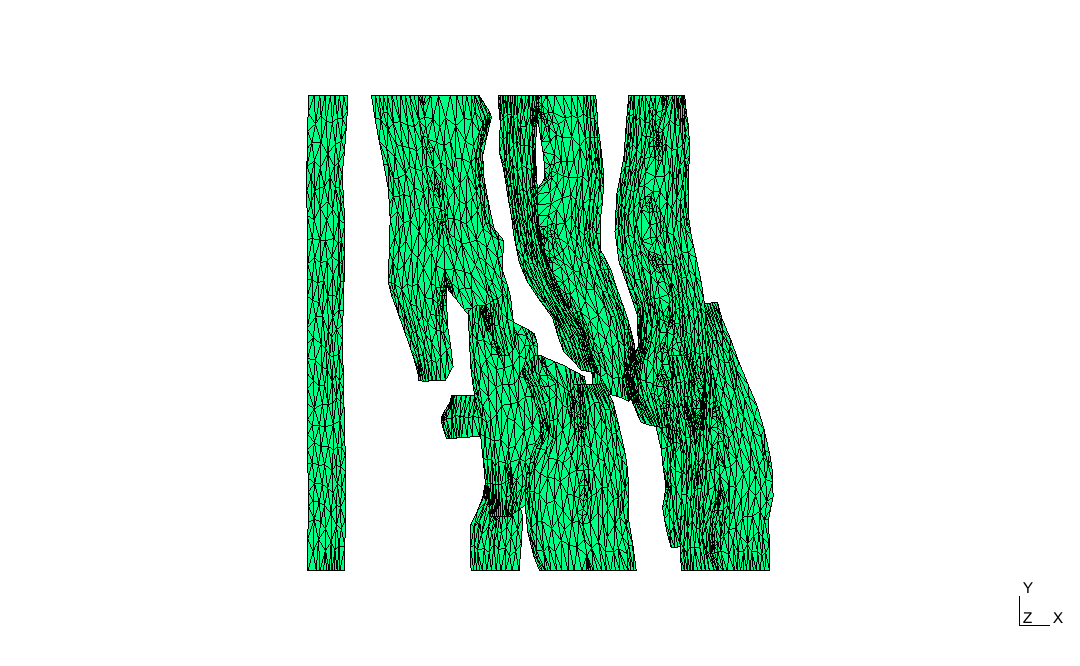
\includegraphics[width=0.35\textwidth]{../images/visu_maillage5364FracsTriangles.png} \quad
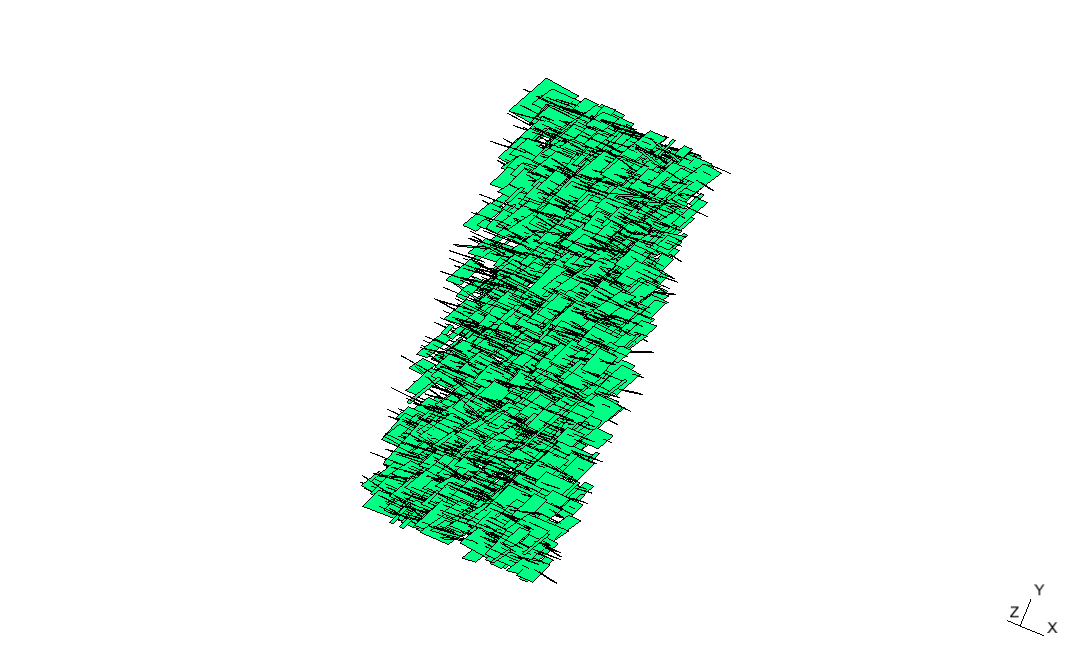
\includegraphics[width=0.25\textwidth]{../images/visu_maillage1994Fracs.png}
\end{figure}

Boundary \emph{integral equation} posed at the surface of cracks

$\Rightarrow$ \alert{dense matrix} $\mA\in \R^{n\times n}$
$\Rightarrow$ $\mathcal{O}(n^{2})$ for matrix-vector product.

\medskip
IFPEN heuristic approach to sparsify $\mA$ gives large error ($16$\%--$40$\%)

\end{frame}

%%%

\begin{frame}
\frametitle{The Elasto$\Phi$ project} 
%\framesubtitle{}

Many refined \emph{complexity reduction} techniques in current literature on boundary integral equation.

\bigskip
Two ingredients in the approach we considered: 
\begin{itemize}
\item
Adaptative Cross Approximation (\alert{ACA}),
\item
Hierarchical Matrices (\alert{HM}).
\end{itemize}

\medskip
Challenge: \emph{strongly irregular geometry!}

\bigskip
\bigskip

{\tiny
[M.~Bebendorf. Hierarchical matrices: A Means to Efficiently Solve Elliptic Boundary Value Problems, {\em Lecture Notes in Computational Science and Engineering}, 2008]

\smallskip
[S.~Rjasanow, O.~Steinbach. The fast solution of boundary integral equations. {\em Mathematical and Analytical Techniques with Applications to Engineering}, 2007]

\smallskip
[W.~Hackbusch. Hierarchical Matrices: Algorithms and Analysis, {\em Springer Series in Computational Mathematics}, 2016]

\smallskip
[S.~A.~Sauter, C.~Schwab. Boundary element methods, {\em Springer Series in Computational Mathematics}, 2011]
\par} %\par per interlinea giusti

\end{frame}

%%%

\begin{frame}
\frametitle{Adaptative Cross Approximation (ACA)}
\framesubtitle{The idea of the Singular Value Decomposition (SVD)} 

\begin{block}{}
Suppose that $\mathrm{A} \in \R^{n\times n}$ is of \alert{low rank}, i.e. 
\[
\mA = \sum_{j=1}^{k}\bfu_{j}\cdot\bfv_{j}^{T}\quad \text{with}\quad \alert{k}\leq n/2.
\]
$\Rightarrow$ \alert{$2kn$} operations for matrix-vector product.
\end{block}


\alert{SVD} actually gives the following decomposition:
\[
\mA = \sum_{j=1}^{n}\sigma_{j}\,\bfu_{j}\cdot\bfv_{j}^{T}\quad \text{ where }\{\sigma_{j}^{2}\}_{j=1\dots n} \text{ are the eigenvalues of } \mA^{T}\mA.
\]

\emph{If} the $\sigma_{j}$ decrease fast, \emph{truncated SVD} is a good approximation of $\mA$!

\medskip
But it costs $\mathcal{O}(n^{3})$ ...

\end{frame}

%%%

\begin{frame}
\frametitle{Adaptative Cross Approximation (ACA)}
\framesubtitle{An approximation of the Singular Value Decomposition} 
\begin{algorithm}[H]
  \caption{Partially Pivoted ACA}  
  Initialize $j_{*}$\\
  $r=0$\\
  \textbf{while}(stopping criterion not satisfied)\{\\
  \indent\hspace{0.5cm} \parbox{\linewidth}{
    $\bfw = \mA(j_{*},:)^{T} - \sum_{\ell=1}^{r}\bfu_{\ell}(j_{*})\,\bfv_{\ell}$\\
    $k_{*} = \mathop{\mrm{argmax}}_{k = 1\dots n}\vert \bfw(k)\vert$\\
    $w_{*} = \bfw(k_{*})$\\
    \textbf{if}($w_{*}\neq 0$)\{\\\quad\\
    \indent\hspace{0.5cm} \parbox{\linewidth}{
      $\bfv_{r+1} = \bfw$\\
      $\bfw = \mA(:,k_{*})-\sum_{\ell = 1}^{r}\bfv_{\ell}(k_{*})\,\bfu_{\ell} $\\
      $\bfu_{r+1} = w_{*}^{-1}\bfw$\\      
      $j_{*} = \mathop{\mrm{argmax}}_{j = 1\dots n} \vert \bfw(j)\vert$\\
      $r=r+1$
    }
   \}\\
    \textbf{else}\{terminate algorithm\}
    }\\
  \}

\end{algorithm}

\end{frame}

%%%

\begin{frame}
\frametitle{Adaptative Cross Approximation (ACA)}
\framesubtitle{Comparaison between SVD and ACA} 
Compression of the interaction matrix between \emph{two clusters} $\{ \bx_i\}$ and $\{ \by_j\}$
\begin{figure}
	\centering 
	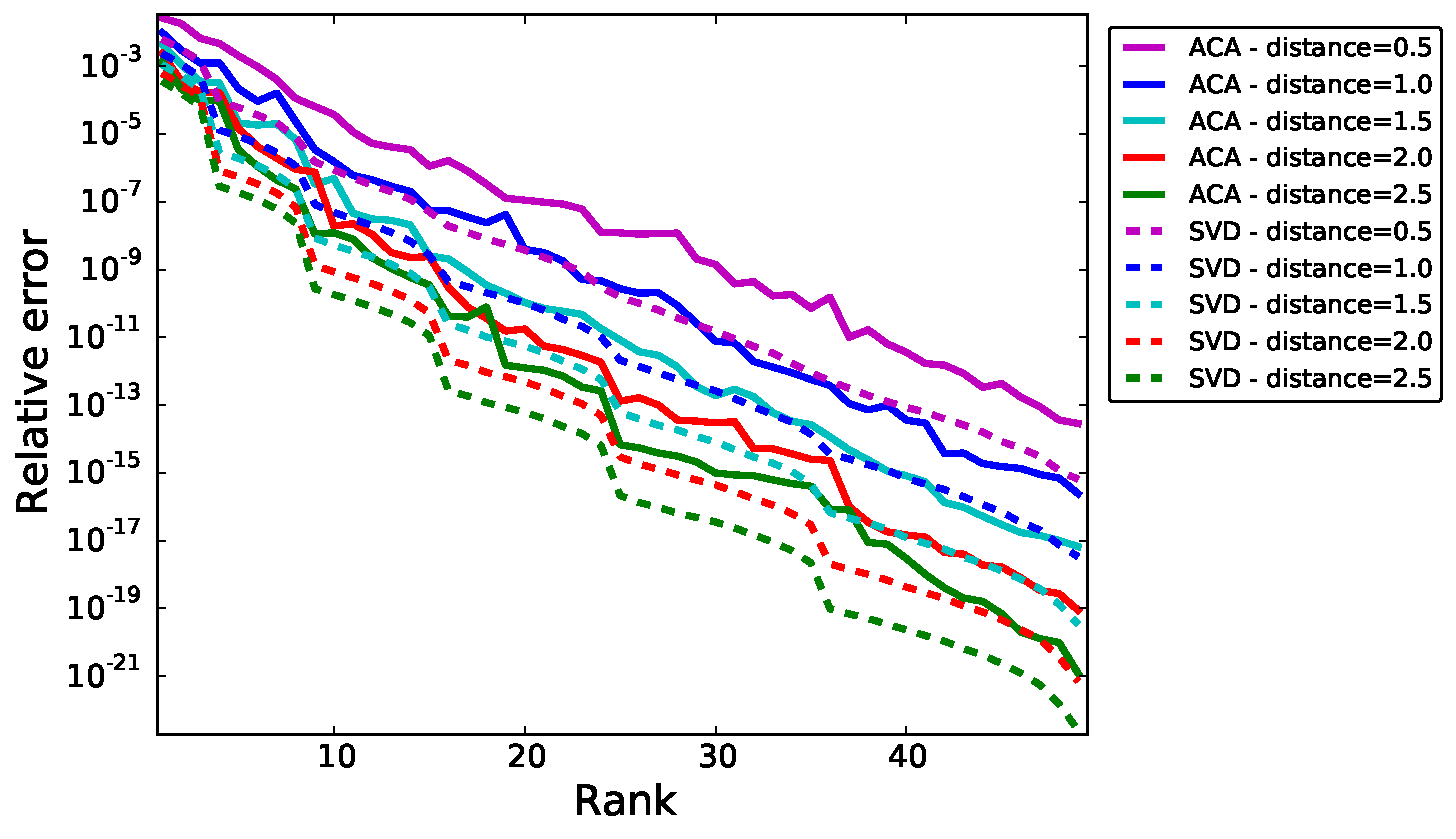
\includegraphics[width=0.9\textwidth]{../images/graphe_output_err_decrease}
\end{figure}

\begin{textblock*}{50mm}(93mm,70mm)
$\mA_{i,j}=\dfrac{1}{4 \pi \Vert\bx_i - \by_j \Vert }$
\end{textblock*}

\end{frame}

%%%

\begin{frame}
\frametitle{Adaptative Cross Approximation (ACA)}
\framesubtitle{In practice in our application} 
The matrix comes from the discretization of a boundary integral equation 
\begin{equation*}\label{GalerkinMatrix}
\mA_{j,k}:= \int_{\tau\times\tau'} \alert{\mathscr{G}(\bx-\by)} \bpsi_{j}(\bx)\bpsi_{k}(\by) d\sigma(\bx) d\sigma(\by),\quad j,k = 1\dots n.
\end{equation*}
\alert{$\mathscr{G}$} is an \emph{integral kernel} with these properties:
\begin{itemize}
\item it is \emph{singular} for $\bx = \by$, i.e.~if $\tau \cap \tau' \ne \emptyset$,
\item it is \emph{regularizing} if $\tau$ and $\tau'$ are \alert{distant} from each other. 
\end{itemize}

\bigskip
 $\Rightarrow$ ACA is applicable to \alert{admissible blocks} of $\mA$
 
 \medskip
 $\Rightarrow$ Hierarchical Matrices (HM)
\end{frame}

%%%

\begin{frame}
\frametitle{Hierarchical matrices}
\framesubtitle{An example of cluster tree en 1D}
We build a cluster tree representing the unknowns, example:
\begin{figure}
	\centering
	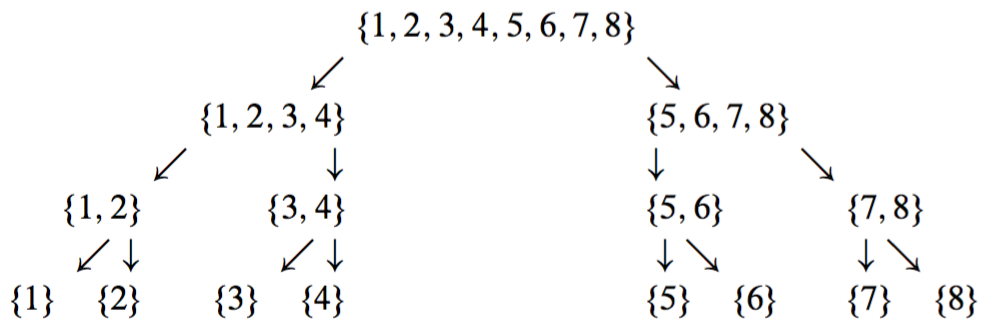
\includegraphics[scale=0.3]{../images/clustering}
\end{figure}

\end{frame}

%%%

\begin{frame}
\frametitle{Hierarchical matrices}
\framesubtitle{An example of cluster tree }
We build a cluster tree representing the unknowns, example:
\begin{figure}
	\centering
	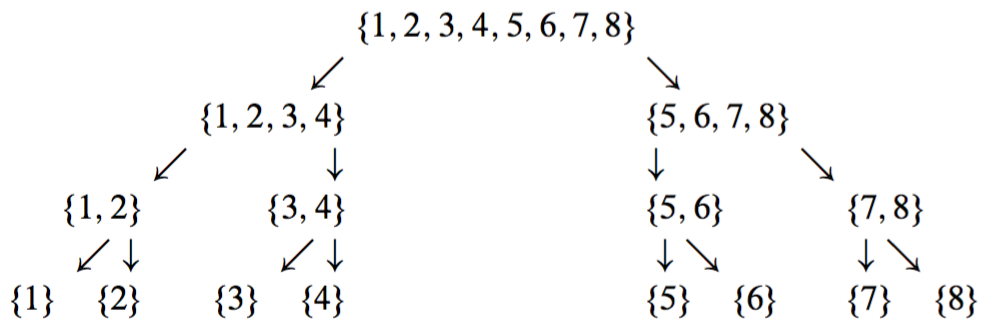
\includegraphics[scale=0.3]{../images/clustering}
	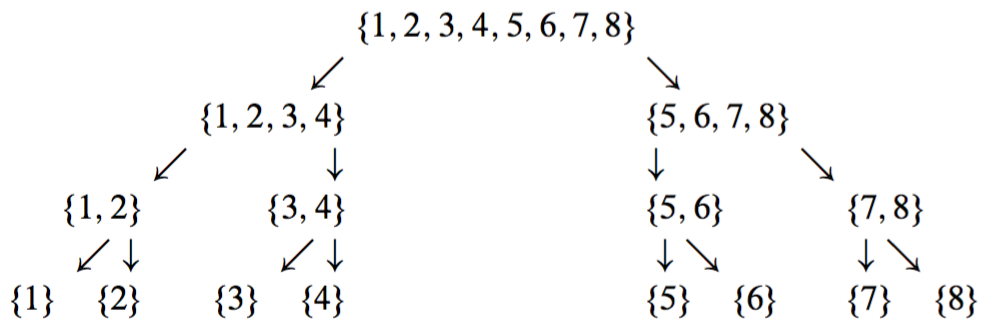
\includegraphics[scale=0.3]{../images/clustering}
\end{figure}
\end{frame}

%%%

\begin{frame}
\frametitle{Results}

C++ implementation, our source code available on GitHub at:
\begin{center}
\url{https://github.com/xclaeys/ElastoPhi}
\end{center}

Varying the parameters of the algorithm:
\vspace{-5pt}
\begin{figure}
\centering
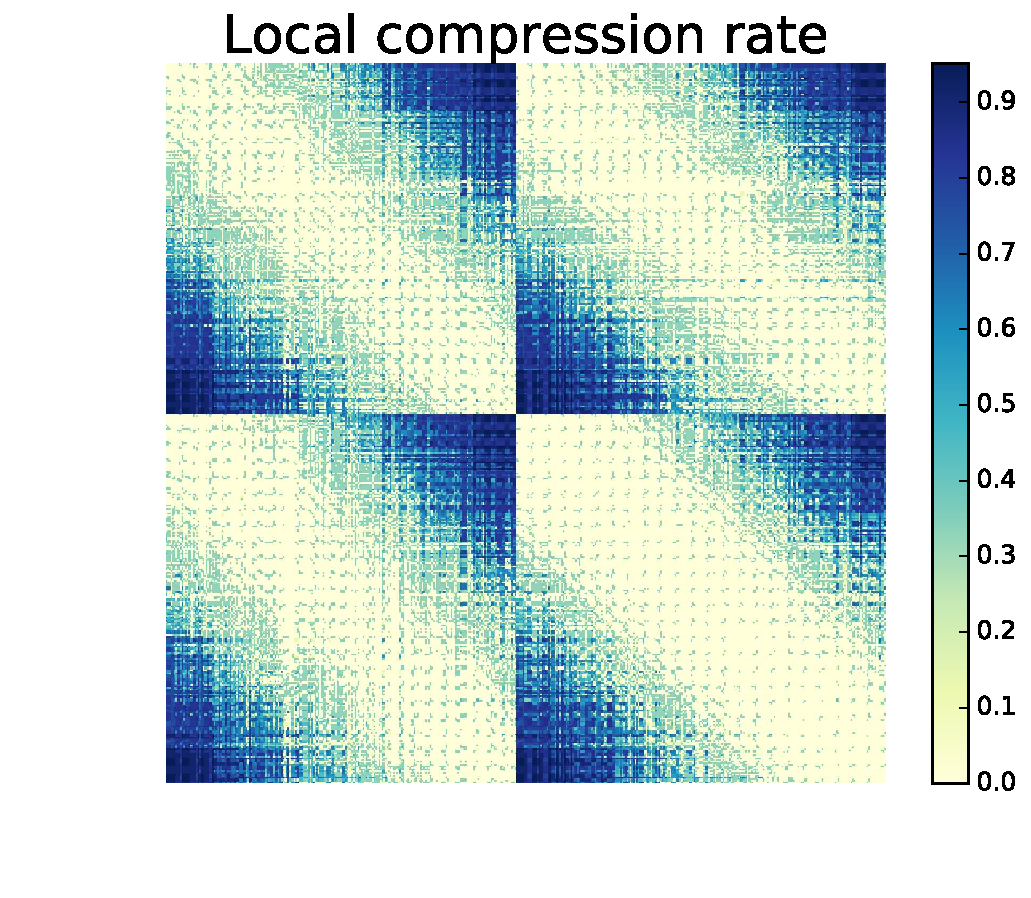
\includegraphics[width=.33\textwidth]{../images/graphe_mapp_output_local_comp_1_0,9_matrice450Fracs.pdf}
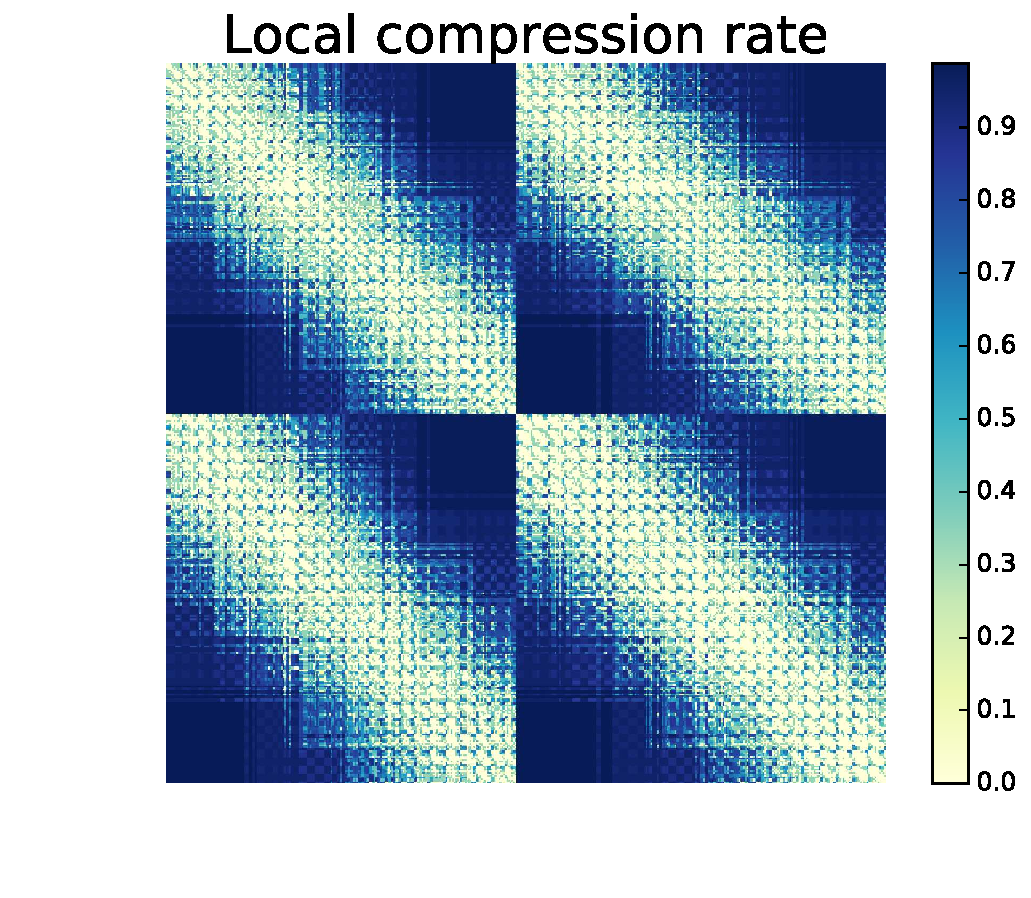
\includegraphics[width=.33\textwidth]{../images/graphe_mapp_output_local_comp_10_0,9_matrice450Fracs.pdf}
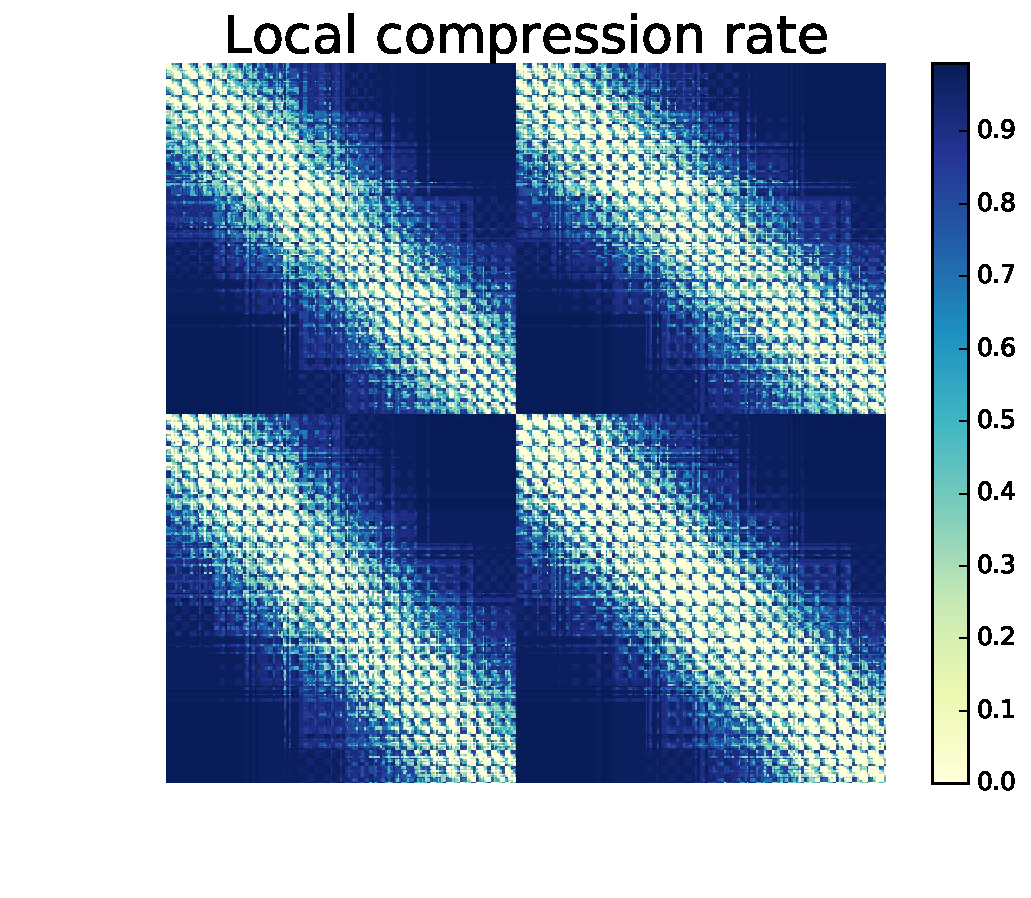
\includegraphics[width=.33\textwidth]{../images/graphe_mapp_output_local_comp_10_1_matrice450Fracs.pdf}
\end{figure}

(A block is not necessarily a connected part of the matrix)
\end{frame}

%%%

\begin{frame}
\frametitle{Results}

\small

Network of $N=1994$ fractures ($3N\times 3N$ matrix $\mA$):
\vspace{-5pt}
\begin{figure}
\centering
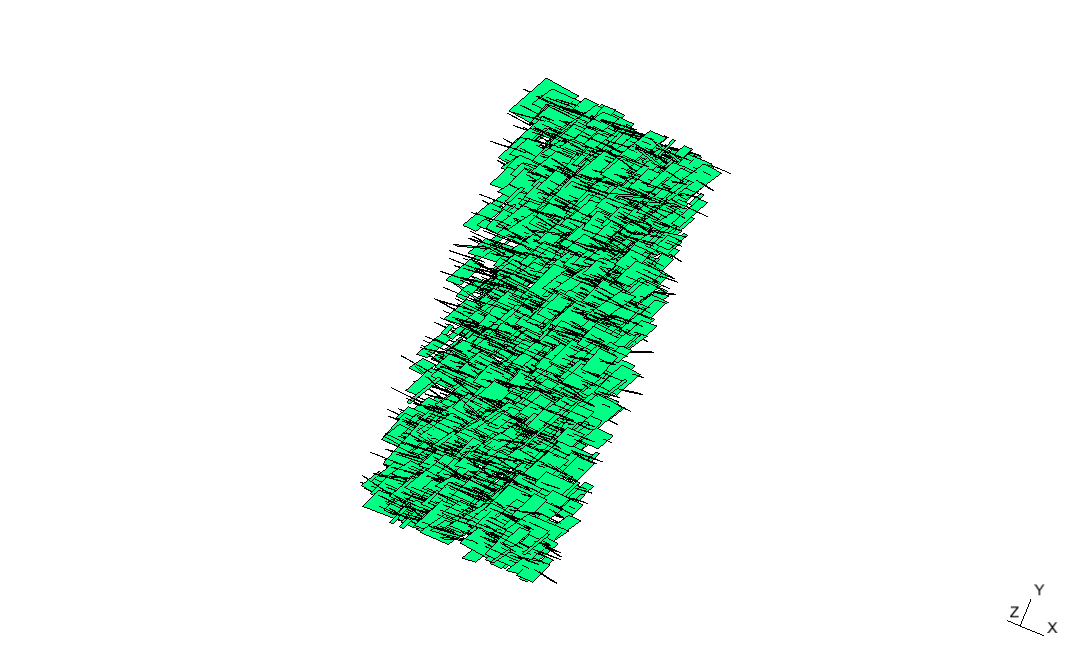
\includegraphics[width=.3\textwidth]{../images/visu_maillage1994Fracs.png}
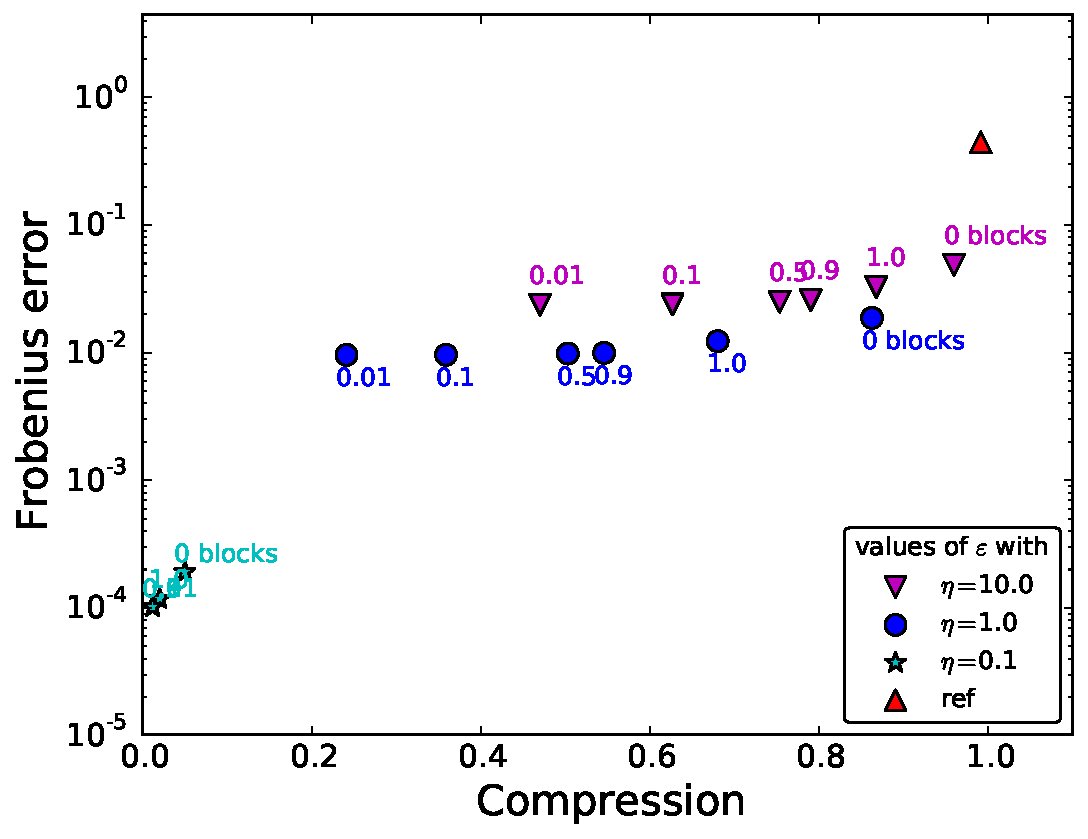
\includegraphics[width=.6\textwidth]{../images/graphe_compasparse_output_compression_18_08_2016matrice1994Fracs.pdf}
\end{figure}

\vspace{-5pt}
{\footnotesize
IFPEN sparse matrix: compression rate $=0.99$, error $=45\%$

H matrix, zero blocks and $\eta=1$: compression rate $=0.86$, error $=2\%$

HM-ACA matrix, $\varepsilon=1$ and $\eta=1$: compression rate $=0.68$, error $=1\%$}

\end{frame}

%%%













\end{document}
